%
% fig-wurzel2.tex
%
% (c) 2026 Prof Dr Andreas Müller
%
\begin{figure}
\centering
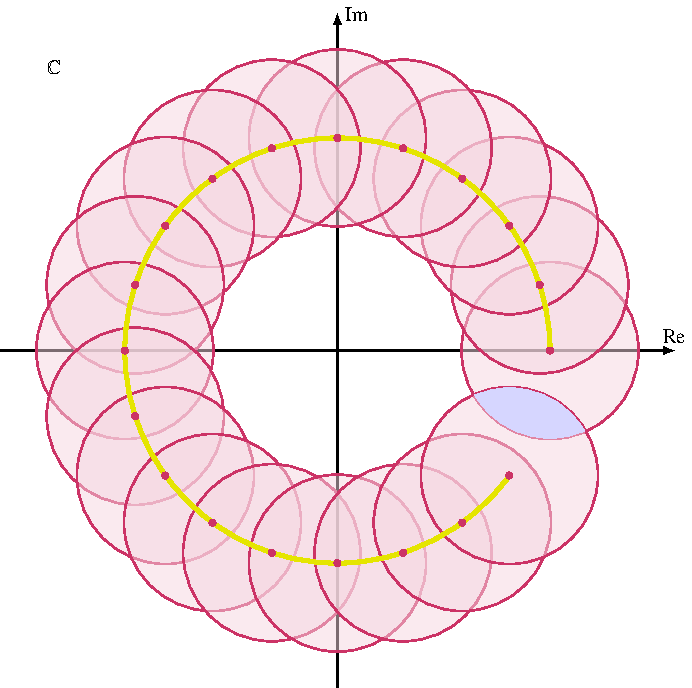
\includegraphics{chapters/040-analytisch/images/wurzel2.pdf}
\caption{Die analytische Fortsetzung der Wurzelfunktion
$f(z)=\!\sqrt{z\mathstrut}$
entlang der gelben Kurve führt im blauen Bereich auf eine
widersprüchliche Definition.
Abbildung~\ref{buch:analytisch:fortsetzung:fig:wurzel} zeigt,
wie durch Konstruktion eines grösseren Definitionsbereichs eine
widerspruchsfreie der Wurzelfunktion gewonnen werden kann.
\label{buch:analytisch:fortsetzung:fig:wurzel2}}
\end{figure}
